\section{内骨格型柔軟グリッパ}
本研究で用いた内骨格型柔軟グリッパを\refig{gripper}
\subsection{柔軟指}
本研究で提案する柔軟指を\refig{soft_finger}に示す.柔軟部にラティス構造を有している.ラティス構造に関しては次の項目で詳しく述べる.3Dプリンタで作成した.使用した3DプリンタはKEYENCE製AGILISTA-3200(\refig{agilista})を用いた.材質はAR-G1H(高硬度シリコン)とした.

\subsection{ラティス構造}
ラティス構造とは\refig{latice}に示す最小の繰り返し単位が周期的に繰り返される3次元構造で、機械的な強度を損なうことなく軽量化を可能とする\cite{latice}.ラティス構造の特徴として3次元構造の形状や周期のパラメータを変更することができ変形量や内部応答を制御することが可能である.本研究ではAutodesk社製のNetfabbを用いてラティス構造の作成を行いその時のパラメータを以下に示す.

\begin{figure}[h]
 \begin{center}
  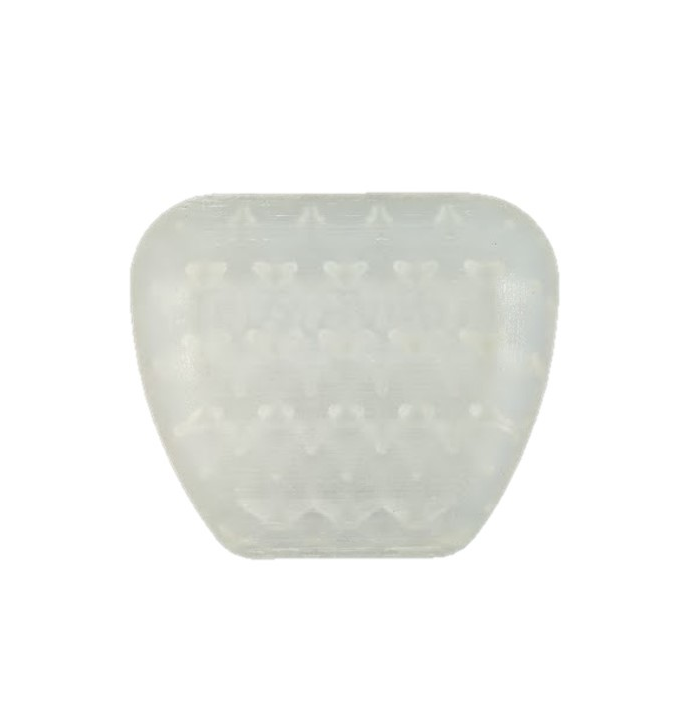
\includegraphics[scale=0.6]{../fig/eps/soft_finger.eps}
 \caption{柔軟指}
  \label{fig::soft_finger}
 \end{center}
\end{figure}

\begin{figure}[b]
 \begin{center}
  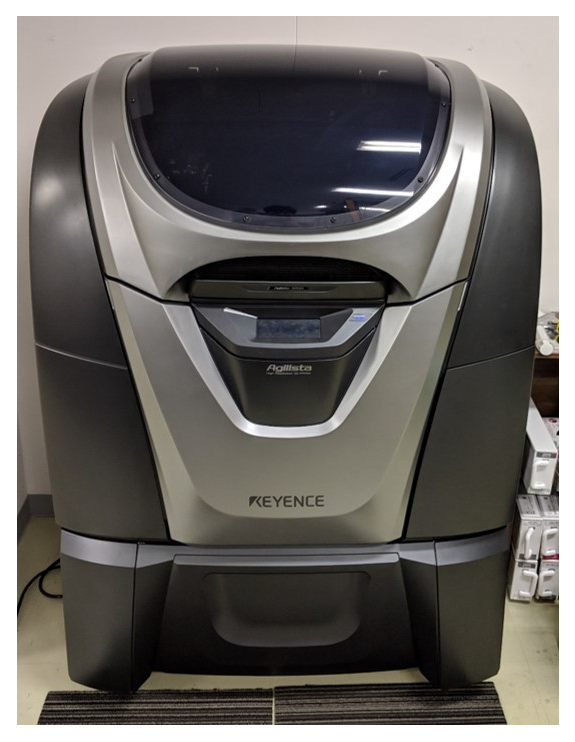
\includegraphics[scale=0.4]{../fig/eps/agilista.eps}
 \caption{KEYENCE製AGILISTA-3200}
  \label{fig::agilista}
 \end{center}
\end{figure}

%\begin{figure}[h]
%\centering
%\subfloat[把持対象物A]{\includegraphics[scale=0.4]{../figure/result_a.eps}}
%\hspace{5mm}
%\subfloat[把持

\subsection{力覚センサ}
イナバゴム社のイナストマーを用いた.\refig{ina}に示す.イナストマーは感圧導電性エラストマー(加圧導電性ゴム)\cite{kanatsu}というゴムを利用した力覚センサである.絶縁性の高いゴム材料(1015~1018Ω)に導電性粒子(カーボン、金属粉、金属蒸着粉等)を一定の配合割合でほぼ均一に混ぜることで感圧導電性を付加している。

\subsubsection{動作原理}



\newpage

	
